\documentclass[11pt,a4paper]{article}  % Déclare la classe du document.

\newcommand{\chaptermark}[2]{\og #2 \fg{} (#1)} % ligne uniquement pour éviter une erreur en cas d'article
\include{../1ere-preambule}

\usepackage{epic}   % extension et simplification de  l'environnement picture
\usepackage{graphicx}    % permet d'inclure des graphique externe dans un document
\usepackage{arydshln}   %permet d'avoir des lignes en pointillés

\newcommand{\lignes}[1]{
	\setlength{\unitlength}{1mm}
	\vskip 0,4cm\noindent
	\multido{\i=0+1}{#1}{%
		\noindent
		\begin{picture}(150,5)
			\linethickness{0,005mm}
			\put(-5,0){\dashline{1}(175,5)(5,5)}
		\end{picture}\vskip 0,001cm
	}
	\vskip 0cm
}

\rhead{\textcolor{red}{Correction - DS n$^{\circ}03$ - Croissance Linéaire - Fonction affine - 10/02/2025}}

\newcommand{\va}[1]{\lvert \ #1 \ \rvert}
\newcommand{\vaf}[1]{\left\lvert \ #1\  \right\rvert}

\begin{document}
	\graphicspath{{images/}}
	
	\begin{center}
		
		
		\fbox{
			\begin{minipage}[]{15cm}
				\begin{center}
					\LARGE{\rule{0.5cm}{0pt}\rule[-0.25cm]{0pt}{0.9cm}
						\textcolor{red}{Correction - DS n$^{\circ}03$ - 10/02/2025 \\
						Croissance Linéaire - Fonction affine} 
					}
				\end{center}
			\end{minipage}
		}
	\end{center}

%\begin{center}\textbf{1h20min - Barème indicatif}\end{center}
%\begin{center}\textbf{Les élèves avec un tier-temps ne traitent pas les questions avec  le symbole \ding{46}}\end{center}
%\begin{center}\textbf{Calculatrice autorisée.\\Les résultats devront être justifiés (à l'aide de calcul ou de propriétés).}\end{center}


\exerciceDS{ - (3 points)}

Soit $f$ la fonction affine définie pour tout réel $x$ par $f(x)=3 x-7$.
\begin{enumMet}
	\item Déterminer $f(-3)$. \corr{$f(-3)=3 \times (-3)-7=-16$}
	\item Quelle est l'image de 5 par $f$ ? \corr{$f(5)=3 \times 5-7=8$}
	\item Résoudre $f(x)=4$. \corr{$f(x)=4 \iff 3 x-7=4 \iff 3x=11 \iff x=\dfrac{11}{3}$}
	\item \ding{46} Déterminer le ou les antécédents de 7 par $f$. \corr{$f(x)=7 \iff 3 x-7=7 \iff 3x=14 \iff x=\dfrac{14}{3}$}
\end{enumMet}

\exerciceDS{ \ding{46} - (3 points)}
La fonction $f$ est une fonction dont la représentation graphique est la droite $(A B)$ et la fonction $g$ une fonction dont la représentation graphique est la droite (CD). 

\ding{46} Par lecture graphique, exprimer $f(x)$ et $g(x)$ en fonction de $x$.

\begin{corrBox}
$$f(x)=\dfrac{1}{2}x-1$$
$$g(x)=-\dfrac{2}{5}x+b$$
La courbe représentative de g passe par C donc : $3=-\dfrac{2}{5}\times 1+b \iff b=\dfrac{17}{5}$
$$g(x)=-\dfrac{2}{5}x+\dfrac{17}{5}$$
	
\end{corrBox}

\begin{center}
	\newrgbcolor{xdxdff}{0.49019607843137253 0.49019607843137253 1.}
	\newrgbcolor{ududff}{0.30196078431372547 0.30196078431372547 1.}
	\newrgbcolor{qqzzqq}{0. 0.6 0.}
	\psset{xunit=1.0cm,yunit=1.0cm,algebraic=true,dimen=middle,dotstyle=o,dotsize=5pt 0,linewidth=1.2pt,arrowsize=3pt 2,arrowinset=0.25}
	\begin{pspicture*}(-1.5,-2.8)(7.8,4.2)
		\multips(0,-2)(0,1.0){8}{\psline[linestyle=dashed,linecap=1,dash=1.5pt 1.5pt,linewidth=0.4pt,linecolor=lightgray]{c-c}(-1.5,0)(7.8,0)}
		\multips(-1,0)(1.0,0){10}{\psline[linestyle=dashed,linecap=1,dash=1.5pt 1.5pt,linewidth=0.4pt,linecolor=lightgray]{c-c}(0,-2.8)(0,4.2)}
		\psaxes[labelFontSize=\scriptstyle,xAxis=true,yAxis=true,Dx=1.,Dy=1.,ticksize=-2pt 0,subticks=2]{->}(0,0)(-1.5,-2.8)(7.8,4.2)
		\psplot[linewidth=1.3pt,linecolor=red]{-1.5}{7.8}{(-4.--2.*x)/4.}
		\psplot[linewidth=1.3pt,linecolor=qqzzqq]{-1.5}{7.8}{(--17.-2.*x)/5.}
%		\begin{scriptsize}
			\psdots[dotstyle=x,linecolor=xdxdff, linewidth=8pt,dotsize=10pt](0.,-1.)
			\rput[bl](0.22,-1.4){\xdxdff{$A$}}
			\psdots[dotstyle=x,linecolor=ududff, linewidth=8pt,dotsize=10pt](4.,1.)
			\rput[bl](4.08,1.2){\ududff{$B$}}
			\rput[bl](-1.4,-1.5){\red{$f$}}
			\psdots[dotstyle=x,linecolor=ududff, linewidth=8pt,dotsize=10pt](1.,3.)
			\rput[bl](1.08,3.2){\ududff{$C$}}
			\psdots[dotstyle=x,linecolor=ududff, linewidth=8pt,dotsize=10pt](6.,1.)
			\rput[bl](6.08,1.2){\ududff{$D$}}
			\rput[bl](-1.4,3.64){\qqzzqq{$g$}}
%		\end{scriptsize}
	\end{pspicture*}
\end{center}

\exerciceDS{ - (2 points)}
On a représenté ci-dessous, par une droite, une fonction g. Exprimer $g(x)$ en fonction de $x$.

\begin{center}
	\newrgbcolor{ududff}{0.30196078431372547 0.30196078431372547 1.}
	\psset{xunit=1.0cm,yunit=1.0cm,algebraic=true,dimen=middle,dotstyle=o,dotsize=5pt 0,linewidth=1.2pt,arrowsize=3pt 2,arrowinset=0.25}
	\begin{pspicture*}(-1.7,-0.5)(13.5,2.8)
		\multips(0,0)(0,1.0){4}{\psline[linestyle=dashed,linecap=1,dash=1.5pt 1.5pt,linewidth=0.4pt,linecolor=lightgray]{c-c}(-1.7,0)(13.5,0)}
		\multips(-1,0)(1.0,0){16}{\psline[linestyle=dashed,linecap=1,dash=1.5pt 1.5pt,linewidth=0.4pt,linecolor=lightgray]{c-c}(0,-0.5)(0,2.8)}
		\psaxes[labelFontSize=\scriptstyle,xAxis=true,yAxis=true,Dx=1.,Dy=1.,ticksize=-2pt 0,subticks=2]{->}(0,0)(-1.7,-0.5)(13.5,2.8)
		\psplot[linewidth=1.3pt,linecolor=red]{-1.7}{13.5}{(--6.--1.*x)/9.}
%		\begin{scriptsize}
			\psdots[dotstyle=x,linecolor=ududff, linewidth=8pt,dotsize=10pt](12.,2.)
			\psdots[dotstyle=x,linecolor=ududff, linewidth=8pt,dotsize=10pt](3.,1.)
			\rput[bl](-0.8,0.7){\red{$g$}}
%		\end{scriptsize}
	\end{pspicture*}
\end{center}

\begin{corrBox}
	par lecture graphique : $a=\dfrac{1}{9}$
	
	La courbe représentative de g passe par $(3;1)$ donc : $1=\dfrac{1}{9}\times 3+b \iff b=1-\dfrac{1}{3}=\dfrac{2}{3}$
	$$g(x)=\dfrac{1}{9}x+\dfrac{2}{3}$$	
\end{corrBox}


\exerciceDS{ - (4 points)}

La fonction $f$ est une fonction affine dont la représentation graphique passe par les points $A(2 ; 9)$ et $B(10 ;-3)$.
\begin{enumMet}
	\item Déterminer une expression de $f(x)$ en fonction de $x$.
	\begin{corrBox}
		$a=\dfrac{y_B-y_A}{x_B-x_A}=\dfrac{-3-9}{10-2}=-\dfrac{12}{8}=-\dfrac{3}{2}$ donc $f(x)=-\dfrac{3}{2}x+b$
		
		La courbe représentative de f passe par A donc: $9=-\dfrac{3}{2}\times 2+b \iff 9=-3+b \iff b=12$
		
		$f(x)=-\dfrac{3}{2}x+12$		
	\end{corrBox}
	\item Calculer $f(4)$. \corr{$f(4)=-\dfrac{3}{2}\times (-4)+12=18$}
	\item Le point de coordonnées $(6 ; 3)$ appartient-il à la courbe représentative de $f$ ?
	\begin{corrBox}
		$f(6)=-\dfrac{3}{2}\times 6+12=3$. On retrouve l'ordonnée du point donc il appartient à la courbe.		
	\end{corrBox}
	
\end{enumMet}
\exerciceDS{ - (1,5 points)}

Parmi les fonctions affines définies ci-dessous, entourer celles qui sont strictement décroissantes sur $\mathbb{R}$.
\renewcommand\fbox{\fcolorbox{red}{white}}
\begin{multicols}{3}
	\begin{enumMet}
		\item \fbox{$f(x)=-\dfrac{1}{4} x+1$}
		\item $f(x)=5 x+3$
		\item \fbox{$f(x)=5-4x$}
		\item $f(x)=-7$
		\item $f(x)=-2+x$
		\item \fbox{$f(x)=-6 x$}
	\end{enumMet}
\end{multicols}

\exerciceDS{ - (3 points)}

Soit $g$ la fonction définie pour tout nombre réel $x$ par $g(x)=8-\dfrac{x}{3}$.
\begin{enumMet}
	\item Déterminer le sens de variation de $g$.
	\begin{corrBox}
		$a=-\dfrac{1}{3}<0$ donc la fonction $g$ est décroissante sur \R.		
	\end{corrBox} 
	\item Comparer les valeurs de $g(54)$ et $g(58)$ sans les calculer.
	\begin{corrBox}
		On a $54<58$ et $g$ décroissante sur \R. Or une fonction décroissante renverse l'ordre donc $g(54)\geqslant g(58)$		
	\end{corrBox}
	\item Déterminer le signe de $g(x)$ selon les valeurs de $x$.
	\begin{corrBox}
		$g(x)=0 \iff 8-\dfrac{x}{3}=0 \iff \dfrac{x}{3}=8 \iff x=8\times 3=24$
		
		\begin{tikzpicture}
			\tkzTabInit{$x$ / 1 , $f(x)$ / 1}{$-\infty$, $24$, $+\infty$}
			\tkzTabLine{, +, z, -, }
		\end{tikzpicture}		
	\end{corrBox}
\end{enumMet}

\exerciceDS{ - (5 points)}

Soit $f$ une fonction affine dont la représentation graphique passe par les points $A(3 ; -4)$ et $B(14 ; 4)$.
\begin{enumMet}
	\item Déterminer une expression de $f(x)$ en fonction de $x$.
	\begin{corrBox}
		$a=\dfrac{y_B-y_A}{x_B-x_A}=\dfrac{4-(-4)}{14-3}=\dfrac{8}{11}$ donc $f(x)=\dfrac{8}{11}x+b$
		
		La courbe représentative de f passe par A donc:
		
		$-4=\dfrac{8}{11}\times 3+b \iff -\dfrac{44}{11}-\dfrac{24}{11}=b \iff b=-\dfrac{68}{11}$
		
		$f(x)=\dfrac{8}{11}x-\dfrac{68}{11}$		
	\end{corrBox}
	\item Calculer $f(5)$.\corr{$f(5)=\dfrac{8}{11}\times 5-\dfrac{68}{11}=-\dfrac{28}{11}$} 
	\item Le point $C\left(\dfrac{5}{4} ; -\dfrac{26}{5}\right)$ appartient-t-il à la courbe représentative de $f$ ?
	\begin{corrBox}
		$f\left(\dfrac{5}{4}\right)=\dfrac{8}{11}\times \dfrac{5}{4}-\dfrac{68}{11}=\dfrac{10}{11}-\dfrac{68}{11}=-\dfrac{58}{11}\neq -\dfrac{26}{5}$. On ne retrouve pas l'ordonnée du point donc le point C n'appartient pas à la courbe.		
	\end{corrBox}
\end{enumMet}

\end{document}
